\documentclass[11pt]{amsart}
\usepackage[margin=1.15in]{geometry}
\usepackage[T1]{fontenc}
\usepackage{lmodern}
\usepackage{amssymb}
\usepackage{booktabs}
\usepackage{tikz}
\usepackage{xcolor}
\usepackage{alltt}
\usepackage[hidelinks]{hyperref}

\definecolor{riverc}{HTML}{1E8F84}
\definecolor{roadc}{HTML}{CDBF9C}
\definecolor{bridgec}{HTML}{D98A1C}
\tikzset{
  river/.style={draw=riverc, line width=1.1pt, line cap=round, line join=round},
  road/.style={fill=roadc!55},
  bridge/.style={fill=bridgec},
}

\raggedbottom
\newcommand{\kw}[1]{\textbf{#1}}
\newenvironment{leancode}{\par\smallskip\noindent\begin{minipage}{\linewidth}\begin{alltt}\small}{\end{alltt}\end{minipage}\par\smallskip}

\newtheorem{theorem}{Theorem}[section]
\newtheorem{proposition}[theorem]{Proposition}
\newtheorem{lemma}[theorem]{Lemma}
\theoremstyle{definition}
\newtheorem{definition}[theorem]{Definition}
\theoremstyle{remark}
\newtheorem{remark}[theorem]{Remark}

\newcommand{\Open}{\mathrm{M}}
\newcommand{\Closed}{\overline{\mathrm{M}}}
\newcommand{\code}[1]{\texttt{#1}}

\title{Counting Arnold's meanders with verified algorithms}
\author{Alexy Khrabrov}
\address{QueryGraph}
\date{October 2026}

\begin{document}

\begin{abstract}
In 1988 V.~I.~Arnold asked in how many ways a river can cross a straight road $n$ times.
No closed formula for these \emph{meander numbers} is known, and the values are known only
by computer enumeration. We formalize the problem in the Lean~4 proof assistant and give two
counting algorithms that are proved, for every $n$, to return exactly the number defined by
the specification. The first is a depth-first search over crossing orders with a pruning rule
based on a parity argument. The second is a transfer matrix that scans the road from west to
east, tracks how the open strands of the river connect, merges equal states, and discards
states that can no longer be completed. Its correctness proof is a bijection between the
action sequences it accepts and meanders, established through a decorated version of the
machine that carries the actual pieces of river. Along the way we prove that closed meanders
of order $n$ are equinumerous with open meanders with $2n-1$ crossings, and that there are at
most $C_n^2$ closed meanders, where $C_n$ is the $n$-th Catalan number. The verified transfer
matrix computes the meander numbers up to $n=30$ in about half a minute; values up to $n=13$
are checked by the Lean kernel alone. Unverified parallel implementations of the same machine
in Rust and OxCaml, with each state packed into one machine word, reproduce the published values
up to $n = 50$, and companion notebooks implement the algorithms in Lean, Python and OCaml. The
development is about 5{,}000 lines of Lean and is available at
\url{https://github.com/querygraph/meander}.
\end{abstract}

\maketitle

\section{Introduction}

A \emph{meander} is a non-self-intersecting curve in the plane that crosses a fixed straight
line a prescribed number of times. In a short note on the topology of real algebraic curves,
Arnold~\cite{arnold88} posed the enumeration question in its most vivid form: in how many ways
can a river cross a straight road $n$ times? Two rivers are considered the same if one can be
deformed into the other without changing the order of the crossings along the road and along
the river. The resulting numbers,
\[
  1,\ 1,\ 1,\ 2,\ 3,\ 8,\ 14,\ 42,\ 81,\ 262,\ 538,\ 1828,\ 3926,\ 13820,\ \dots
\]
form sequence A005316 of the OEIS~\cite{oeis-a005316}. The closely related count of closed
curves crossing the line $2n$ times is A005315~\cite{oeis-a005315}. Meanders appeared earlier in
work on folding a strip of stamps~\cite{touchard50}, were studied systematically by Lando and
Zvonkin~\cite{lando-zvonkin}, and became a test bed for exact enumeration and statistical
physics~\cite{dgg97,dgg00,jensen00}.

Despite this attention there is no closed formula. Di~Francesco, Golinelli and Guitter
conjectured from a conformal field theory argument that the number of closed meanders of order
$n$ grows like $C\,R^{2n} n^{-\alpha}$ with $R^2 \approx 12.26$ and
$\alpha = (29+\sqrt{145})/12$~\cite{dgg00}. Rigorous bounds on the growth rate are far apart:
Albert and Paterson proved that the exponential growth constant $R^2$ lies between about
$11.38$ and $12.90$~\cite{albert-paterson}. Every known value of the sequence comes from a
computer program, and the best of these are intricate transfer-matrix
codes~\cite{jensen00}.

This paper asks a narrower question: can we compute meander numbers with programs whose
correctness is machine-checked against the plain definition? We answer it in the Lean~4 proof
assistant~\cite{lean4} with the mathlib library~\cite{mathlib}. Our contributions are:

\begin{enumerate}
  \item A formal specification of open meanders as permutations of the bridges satisfying a
    non-crossing condition, and of closed meanders (Section~\ref{sec:spec}).
  \item Structural theorems: open meanders exist for every $n$; there are at most $n!$; closed
    meanders of order $n$ correspond bijectively to open meanders with $2n-1$ crossings; and
    there are at most $C_n^2$ closed meanders (Section~\ref{sec:structure}).
  \item A depth-first search with a pruning rule derived from a parity argument, proved equal
    to the specification (Section~\ref{sec:search}).
  \item A transfer matrix with state merging and a capacity-based pruning rule, proved equal to
    the specification by a bijection between accepted action sequences and meanders
    (Section~\ref{sec:tm}).
  \item Certified values: kernel-checked for $n \le 13$, and computed by the verified transfer
    matrix up to $n = 32$, matching the OEIS (Section~\ref{sec:values}).
  \item Parallel implementations of the same machine in Rust and OxCaml, unverified but checked
    against the certified values and the OEIS, which reach $n = 50$; teaching implementations in
    Python and OCaml; and a comparison of all of them (Section~\ref{sec:implementations}).
\end{enumerate}

We do not claim new values of the sequence; larger values are known~\cite{jensen00}. What
is new is that the values we report come from programs proved correct for all $n$, and that
the proofs expose the combinatorial facts that make the fast algorithms work.

\section{The specification}\label{sec:spec}

\subsection{From a picture to a permutation}
Label the bridges $0,1,\dots,n-1$ from west to east. Following Arnold, the river enters from
the south and leaves to the east. Between consecutive crossings it runs along an arc in one of
the two half-planes, alternately: the first arc, from the south, lies below the road, the next
above, and so on. A river is therefore determined up to deformation by its \emph{crossing
order}, the permutation $\tau$ with $\tau(i)$ the bridge crossed $i$-th.

Not every permutation is realized. To state the condition, compactify each half-plane to a
disk whose boundary consists of the road and one point at infinity, and record the two ends of
the river as two boundary points east of every bridge: the east end $E = n$ and the south end
$S = n+1$. (Going around the lower disk counterclockwise, one meets the bridges, then east,
then south.) The river's path is the sequence of boundary points
\[
  P_0 = S,\quad P_1 = \tau(0),\ \dots,\ P_n = \tau(n-1),\quad P_{n+1} = E,
\]
and arc $k$ joins $P_k$ and $P_{k+1}$ in the lower half-plane if $k$ is even and the upper one
if $k$ is odd. By the Jordan curve theorem the river is simple exactly when no two arcs on the
same side cross, and two chords of a disk cross exactly when their endpoints alternate around
the boundary. Because all endpoints are now points of a line, alternation is an elementary
condition.

\begin{definition}
Chords $\{a,b\}$ and $\{c,d\}$ \emph{interleave} if exactly one of $c,d$ lies strictly between
$\min(a,b)$ and $\max(a,b)$. A point sequence $P$ has \emph{no crossing among its first $L$
arcs} if for all $j<k<L$ with $j \equiv k \pmod 2$, the arcs $\{P_j,P_{j+1}\}$ and
$\{P_k,P_{k+1}\}$ do not interleave. A permutation $\tau$ of $\{0,\dots,n-1\}$ is an
\emph{open meander} if its path has no crossing among its $n+1$ arcs. We write $\Open_n$ for
the number of open meanders.
\end{definition}

\noindent Figure~\ref{fig:spec} gives the specification in Lean. Figure~\ref{fig:n4} shows the three open meanders with four
crossings, and Figure~\ref{fig:n5} shows all eight with five.

\begin{figure}[t]
\begin{leancode}
\kw{def} Interleave (a b c d : Nat) : Prop :=
  \(\neg\) ((min a b < c \(\wedge\) c < max a b) \(\leftrightarrow\) (min a b < d \(\wedge\) d < max a b))

\kw{def} NoCross (P : Nat \(\to\) Nat) (L : Nat) : Prop :=
  \(\forall\) k < L, \(\forall\) j < k, j % 2 = k % 2 \(\to\)
    \(\neg\) Interleave (P j) (P (j + 1)) (P k) (P (k + 1))

\kw{def} IsMeander \{n : \(\mathbb{N}\)\} (\(\sigma\) : Equiv.Perm (Fin n)) : Prop :=
  NoCross (pathPt \(\sigma\)) (n + 1)

\kw{def} openMeanderCount (n : \(\mathbb{N}\)) : \(\mathbb{N}\) :=
  Fintype.card \{\(\sigma\) : Equiv.Perm (Fin n) // IsMeander \(\sigma\)\}
\end{leancode}
\caption{The specification in Lean~4. \code{pathPt}~$\sigma$ is the point sequence $P$ of the river with crossing order~$\sigma$.}\label{fig:spec}
\end{figure}

\begin{figure}[t]
\centering
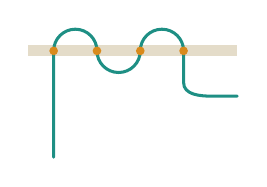
\begin{tikzpicture}[baseline=0pt]
\fill[road] (-0.330,-0.07) rectangle (2.330,0.07);
\draw[river] (0.000,-1.35) -- (0.000,0) arc (180:0:0.275) arc (180:360:0.275) arc (180:0:0.275) -- (1.650,-0.402) to[out=-90,in=180] (2.000,-0.575) -- (2.330,-0.575);
\fill[bridge] (0.000,0) circle (0.055);
\fill[bridge] (0.550,0) circle (0.055);
\fill[bridge] (1.100,0) circle (0.055);
\fill[bridge] (1.650,0) circle (0.055);
\end{tikzpicture}
\hspace{1.2em}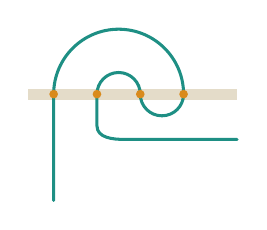
\begin{tikzpicture}[baseline=0pt]
\fill[road] (-0.330,-0.07) rectangle (2.330,0.07);
\draw[river] (0.000,-1.35) -- (0.000,0) arc (180:0:0.825) arc (360:180:0.275) arc (0:180:0.275) -- (0.550,-0.402) to[out=-90,in=180] (0.900,-0.575) -- (2.330,-0.575);
\fill[bridge] (0.000,0) circle (0.055);
\fill[bridge] (0.550,0) circle (0.055);
\fill[bridge] (1.100,0) circle (0.055);
\fill[bridge] (1.650,0) circle (0.055);
\end{tikzpicture}
\hspace{1.2em}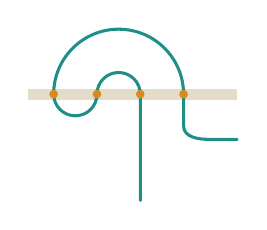
\begin{tikzpicture}[baseline=0pt]
\fill[road] (-0.330,-0.07) rectangle (2.330,0.07);
\draw[river] (1.100,-1.35) -- (1.100,0) arc (0:180:0.275) arc (360:180:0.275) arc (180:0:0.825) -- (1.650,-0.402) to[out=-90,in=180] (2.000,-0.575) -- (2.330,-0.575);
\fill[bridge] (0.000,0) circle (0.055);
\fill[bridge] (0.550,0) circle (0.055);
\fill[bridge] (1.100,0) circle (0.055);
\fill[bridge] (1.650,0) circle (0.055);
\end{tikzpicture}

\caption{The three open meanders with $n=4$ crossings. The river enters from the south and
leaves to the east; bridges are numbered $0$ to $3$ from west to east. Their crossing orders
are $0123$, $0321$ and $2103$.}\label{fig:n4}
\end{figure}

\subsection{Closed meanders}
A closed meander of order $n$ is a simple closed curve crossing the road $2n$ times. To count
each curve once we fix where it starts and in which direction it runs: it starts at the
westmost bridge and leaves it into the upper half-plane. It is then a permutation $\sigma$ of
$\{0,\dots,2n-1\}$ with $\sigma(0)=0$ whose cyclic path has no crossing among its $2n$ arcs.
We write $\Closed_n$ for their number.

\begin{figure}[p]
\centering
\begin{tabular}{cc}
\begin{tabular}{c}\scalebox{1.32}{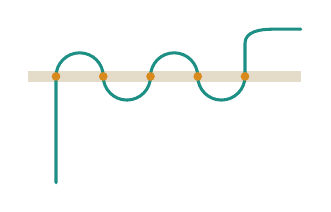
\begin{tikzpicture}[baseline=0pt]
\fill[road] (-0.360,-0.07) rectangle (3.110,0.07);
\draw[river] (0.000,-1.35) -- (0.000,0) arc (180:0:0.300) arc (180:360:0.300) arc (180:0:0.300) arc (180:360:0.300) -- (2.400,0.420) to[out=90,in=180] (2.750,0.600) -- (3.110,0.600);
\fill[bridge] (0.000,0) circle (0.055);
\fill[bridge] (0.600,0) circle (0.055);
\fill[bridge] (1.200,0) circle (0.055);
\fill[bridge] (1.800,0) circle (0.055);
\fill[bridge] (2.400,0) circle (0.055);
\end{tikzpicture}
}\\[4pt] \small $01234$\end{tabular} & \begin{tabular}{c}\scalebox{1.32}{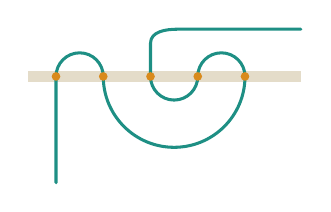
\begin{tikzpicture}[baseline=0pt]
\fill[road] (-0.360,-0.07) rectangle (3.110,0.07);
\draw[river] (0.000,-1.35) -- (0.000,0) arc (180:0:0.300) arc (180:360:0.900) arc (0:180:0.300) arc (360:180:0.300) -- (1.200,0.420) to[out=90,in=180] (1.550,0.600) -- (3.110,0.600);
\fill[bridge] (0.000,0) circle (0.055);
\fill[bridge] (0.600,0) circle (0.055);
\fill[bridge] (1.200,0) circle (0.055);
\fill[bridge] (1.800,0) circle (0.055);
\fill[bridge] (2.400,0) circle (0.055);
\end{tikzpicture}
}\\[4pt] \small $01432$\end{tabular} \\[30pt]
\begin{tabular}{c}\scalebox{1.32}{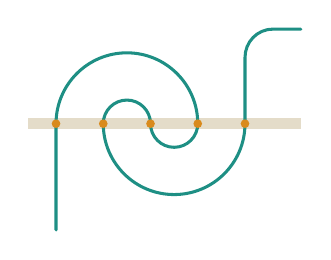
\begin{tikzpicture}[baseline=0pt]
\fill[road] (-0.360,-0.07) rectangle (3.110,0.07);
\draw[river] (0.000,-1.35) -- (0.000,0) arc (180:0:0.900) arc (360:180:0.300) arc (0:180:0.300) arc (180:360:0.900) -- (2.400,0.840) to[out=90,in=180] (2.750,1.200) -- (3.110,1.200);
\fill[bridge] (0.000,0) circle (0.055);
\fill[bridge] (0.600,0) circle (0.055);
\fill[bridge] (1.200,0) circle (0.055);
\fill[bridge] (1.800,0) circle (0.055);
\fill[bridge] (2.400,0) circle (0.055);
\end{tikzpicture}
}\\[4pt] \small $03214$\end{tabular} & \begin{tabular}{c}\scalebox{1.32}{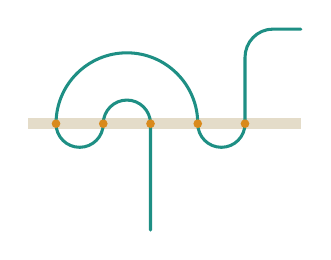
\begin{tikzpicture}[baseline=0pt]
\fill[road] (-0.360,-0.07) rectangle (3.110,0.07);
\draw[river] (1.200,-1.35) -- (1.200,0) arc (0:180:0.300) arc (360:180:0.300) arc (180:0:0.900) arc (180:360:0.300) -- (2.400,0.840) to[out=90,in=180] (2.750,1.200) -- (3.110,1.200);
\fill[bridge] (0.000,0) circle (0.055);
\fill[bridge] (0.600,0) circle (0.055);
\fill[bridge] (1.200,0) circle (0.055);
\fill[bridge] (1.800,0) circle (0.055);
\fill[bridge] (2.400,0) circle (0.055);
\end{tikzpicture}
}\\[4pt] \small $21034$\end{tabular} \\[30pt]
\begin{tabular}{c}\scalebox{1.32}{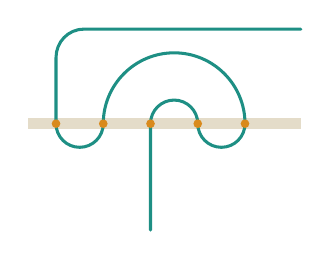
\begin{tikzpicture}[baseline=0pt]
\fill[road] (-0.360,-0.07) rectangle (3.110,0.07);
\draw[river] (1.200,-1.35) -- (1.200,0) arc (180:0:0.300) arc (180:360:0.300) arc (0:180:0.900) arc (360:180:0.300) -- (0.000,0.840) to[out=90,in=180] (0.350,1.200) -- (3.110,1.200);
\fill[bridge] (0.000,0) circle (0.055);
\fill[bridge] (0.600,0) circle (0.055);
\fill[bridge] (1.200,0) circle (0.055);
\fill[bridge] (1.800,0) circle (0.055);
\fill[bridge] (2.400,0) circle (0.055);
\end{tikzpicture}
}\\[4pt] \small $23410$\end{tabular} & \begin{tabular}{c}\scalebox{1.32}{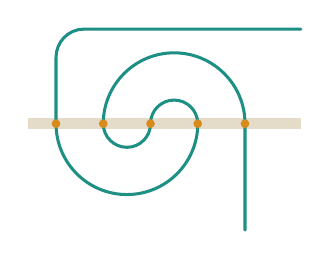
\begin{tikzpicture}[baseline=0pt]
\fill[road] (-0.360,-0.07) rectangle (3.110,0.07);
\draw[river] (2.400,-1.35) -- (2.400,0) arc (0:180:0.900) arc (180:360:0.300) arc (180:0:0.300) arc (360:180:0.900) -- (0.000,0.840) to[out=90,in=180] (0.350,1.200) -- (3.110,1.200);
\fill[bridge] (0.000,0) circle (0.055);
\fill[bridge] (0.600,0) circle (0.055);
\fill[bridge] (1.200,0) circle (0.055);
\fill[bridge] (1.800,0) circle (0.055);
\fill[bridge] (2.400,0) circle (0.055);
\end{tikzpicture}
}\\[4pt] \small $41230$\end{tabular} \\[30pt]
\begin{tabular}{c}\scalebox{1.32}{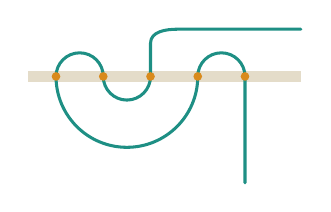
\begin{tikzpicture}[baseline=0pt]
\fill[road] (-0.360,-0.07) rectangle (3.110,0.07);
\draw[river] (2.400,-1.35) -- (2.400,0) arc (0:180:0.300) arc (360:180:0.900) arc (180:0:0.300) arc (180:360:0.300) -- (1.200,0.420) to[out=90,in=180] (1.550,0.600) -- (3.110,0.600);
\fill[bridge] (0.000,0) circle (0.055);
\fill[bridge] (0.600,0) circle (0.055);
\fill[bridge] (1.200,0) circle (0.055);
\fill[bridge] (1.800,0) circle (0.055);
\fill[bridge] (2.400,0) circle (0.055);
\end{tikzpicture}
}\\[4pt] \small $43012$\end{tabular} & \begin{tabular}{c}\scalebox{1.32}{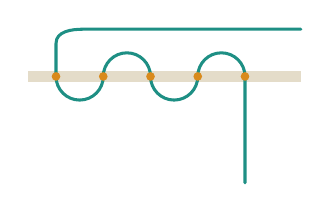
\begin{tikzpicture}[baseline=0pt]
\fill[road] (-0.360,-0.07) rectangle (3.110,0.07);
\draw[river] (2.400,-1.35) -- (2.400,0) arc (0:180:0.300) arc (360:180:0.300) arc (0:180:0.300) arc (360:180:0.300) -- (0.000,0.420) to[out=90,in=180] (0.350,0.600) -- (3.110,0.600);
\fill[bridge] (0.000,0) circle (0.055);
\fill[bridge] (0.600,0) circle (0.055);
\fill[bridge] (1.200,0) circle (0.055);
\fill[bridge] (1.800,0) circle (0.055);
\fill[bridge] (2.400,0) circle (0.055);
\end{tikzpicture}
}\\[4pt] \small $43210$\end{tabular} \\[30pt]
\end{tabular}
\caption{All eight open meanders with $n=5$ crossings, each labelled with its crossing order
(the bridges crossed, in river order, numbered from west to east). The river enters from the
south; since $n$ is odd, its last arc lies above the road and it leaves to the east above
every other upper arc.}\label{fig:n5}
\end{figure}

\clearpage
\section{Structural results}\label{sec:structure}

\begin{theorem}\label{thm:basic}
For every $n$, $0 < \Open_n \le n!$.
\end{theorem}
\begin{proof}[Proof sketch]
The upper bound is the cardinality of a subtype of the permutations. For the lower bound, the
identity permutation is a meander: all its arcs except the first join neighbouring bridges, so
nothing lies strictly between their ends, and the first arc, from $S=n+1$ to bridge $0$,
encloses every other lower arc.
\end{proof}

\begin{theorem}\label{thm:closed-open}
For every $n \ge 1$, $\Closed_n = \Open_{2n-1}$.
\end{theorem}
\begin{proof}[Proof sketch]
Delete the westmost bridge of a closed meander and rotate the picture by $180^\circ$. The two
arcs at the deleted bridge now run off to infinity: one in the lower half-plane, from which the
river enters, and one to the east, where it leaves. The result is an open meander with $2n-1$
crossings, and the construction can be reversed. In coordinates the map sends an open crossing
order $\tau$ on $2n-1$ bridges to the closed order $0,\,2n-1-\tau(0),\,2n-1-\tau(1),\dots$,
which in Lean is $\code{decomposeFin.symm}\,(0, \tau \cdot \code{revPerm})$. Reflection
$x \mapsto 2n-1-x$ reverses the order on the bridges, so it preserves interleaving. The only
subtlety is the south end $2n$, which truncated subtraction sends to the new bridge $0$; it is
an endpoint of a single lower arc, and every other lower arc has both endpoints among the
bridges, so interleaving is unaffected. All of this reduces to \code{omega} once the values of
the path are pinned down.
\end{proof}

\begin{theorem}\label{thm:catalan}
For every $n$, $\Closed_n \le C_n^2$, where $C_n = \frac{1}{n+1}\binom{2n}{n}$.
\end{theorem}
\begin{proof}[Proof sketch]
By Theorem~\ref{thm:closed-open} it suffices to inject open meanders with $2n+1$ crossings into
pairs of Dyck words of semilength $n+1$; mathlib already proves that there are $C_{n+1}$ such
words. Treat the two ends of the river as extra points east of every bridge. Each half-plane
then carries a non-crossing perfect matching of $2n+2$ points, and the river is recovered by
walking from the south end and taking, at each point, the partner on the side where the river
currently is. A non-crossing matching is determined by its \emph{pattern}, the word recording
whether each point opens ($U$) or closes ($D$) its arc. To see this, let $s_i = \pm 1$ according
to the pattern and let $B(x,z) = \sum_{x<i<z} s_i$. For an opener $x$ with partner $y$, every
arc starting strictly inside $(x,y)$ also ends inside it, so $B(x,y) = 0$ and $B(x,z) \ge 0$
for $x < z \le y$. These two facts locate $y$ from the pattern alone: if a second matching with
the same pattern paired $x$ with $y' > y$, then $B(x,y+1) = -1 < 0$, a contradiction. Closers
are handled symmetrically. The pattern is a Dyck word because every closer in a prefix is
matched to an opener in the same prefix.
\end{proof}

\section{A verified search with parity pruning}\label{sec:search}

The specification counts permutations, so evaluating it directly costs $n!$ steps. The first
algorithm builds the crossing order one bridge at a time. It abandons a branch as soon as the
newest arc crosses an earlier arc on the same side, or as soon as the following test fails.

\begin{lemma}[Parity]\label{lem:parity}
Let $q$ be a prefix of a meander, with $t = |q|$ arcs already drawn, and let $j < t$ be one of
them, on side $s = j \bmod 2$, with ends $a<b$. Count the arc ends still to come on side $s$
that lie strictly between $a$ and $b$: every unused bridge in $(a,b)$; the current point, if
the next arc is on side $s$; and the east end, if the last arc is on side $s$. This number is
even.
\end{lemma}
\begin{proof}
Each later arc on side $s$ has both ends inside $(a,b)$ or neither, since it may not cross
arc $j$. Each point listed is the end of exactly one later arc on side $s$, and no other point
is. Formally, an induction along the remainder of the river shows that the running count of
such ends inside $(a,b)$ changes by $0$ or $2$ with each later arc on side $s$.
\end{proof}

The correctness theorem \code{openMeanderCount\_eq\_meanderCount} has two parts. First, the
search equals the number of complete orderings, generated by the same recursion, that satisfy
the specification; this holds because a pruned branch contains no meanders (for crossings, by
monotonicity of \code{NoCross}; for parity, by Lemma~\ref{lem:parity}). Second, permutations of
$\mathrm{Fin}\,n$ correspond bijectively to members of that list of orderings.

Measured in a prototype, parity pruning reduces the number of search nodes at $n=11$ from
$322{,}080$ to $14{,}471$. A further rule, that every remaining bridge be reachable from the
current point through the regions cut out by the drawn arcs, reduces this to $9{,}835$. For
$n \le 10$ the reduced search visits exactly the prefixes of actual meanders, so no further
pruning rule of this kind can help (Table~\ref{tab:nodes}). In the compiled search the
reachability test cost more than it saved, so we did not adopt it; the transfer matrix of the
next section enforces connectivity by construction.

\begin{table}[t]
\centering
\begin{tabular}{rrrrrr}
\toprule
$n$ & $\Open_n$ & crossing test & $+$ parity & $+$ reachability & completable prefixes \\
\midrule
8  & 81    & 6{,}077   & 522     & 404    & 404 \\
9  & 262   & 22{,}452  & 1{,}746  & 1{,}336 & 1{,}336 \\
10 & 538   & 84{,}419  & 4{,}115  & 2{,}854 & 2{,}854 \\
11 & 1{,}828 & 322{,}080 & 14{,}471 & 9{,}835 & --- \\
\bottomrule
\end{tabular}
\caption{Nodes visited by the depth-first search under successive pruning rules, and the
number of prefixes that can actually be completed (a lower bound for any search that builds
the river bridge by bridge).}\label{tab:nodes}
\end{table}

\section{A verified transfer matrix}\label{sec:tm}

\subsection{The machine}
Scan the points of the road from west to east: the bridges, then $E$ (one arc, on side
$n \bmod 2$), then $S$ (one arc, below). Each point \emph{opens} or \emph{closes} its arc on
each of its sides. Arcs on one side never cross, so the arcs still open at a cut form a
\emph{stack} on each side, and a closing point always closes the top of its stack.

To the west of the cut the river is broken into pieces. Each piece joins two open arcs, or an
open arc and the east end. The state records, for every open arc in stack order, a reference to
where its piece leads:
\begin{leancode}
\kw{inductive} Ref \kw{where}
  | E                         \textit{-- the east end}
  | s (\(\sigma\) : Bool) (i : Nat)    \textit{-- position i in the stack of side \(\sigma\)}

\kw{structure} St \kw{where}
  up : List Ref
  dn : List Ref
\end{leancode}
There are four transitions at a bridge. Opening both sides creates a new piece whose two ends
are the two new arcs. Opening one side and closing the other continues the closed arc's piece
along the new arc. Closing both sides joins two pieces, unless the two arcs being closed are
the two ends of the same piece; that would close a loop, so the machine rejects it. At $E$ the
top arc on its side is closed and its piece now ends at $E$, or a new arc is opened towards
$S$. A sequence is accepted when, after $E$, exactly one arc is open, below the road, leading
to $E$, so that $S$ can close it.

\subsection{Counting with merging and pruning}
The machine is run on all action sequences at once, layer by layer. Each layer is a list of
states with multiplicities, and equal states are merged by sorting and adding adjacent
counts. Any merge procedure is admissible if it preserves weighted sums
$\sum_{(s,c)} c\cdot g(s)$ for every weight function $g$; the counting theorem
\code{tmCountWith\_eq\_countP} is proved for an arbitrary such procedure. We instantiate it
twice: with a sort-based merge for compiled execution, and with a structurally recursive
insertion merge that the Lean kernel can evaluate.

Each layer also drops states that cannot be finished. Every remaining point closes at most one
arc on each of its sides, and the accepting state has no open arc above the road and one below,
so a state with more open arcs than the remaining points can close has no accepted
continuation. In a prototype this \emph{viability} test reduces the total number of states over
all layers at $n=17$ from $512{,}350$ to $3{,}135$. Its soundness is an induction showing that
a single step lowers each stack by at most one, and only on the sides the point has.

\subsection{Correctness}
The counting theorem reduces correctness of the transfer matrix to the following statement.

\begin{theorem}\label{thm:tm}
The action sequences accepted by the machine are in bijection with open meanders. Consequently
\code{tmCount m = openMeanderCount m} for every $m$.
\end{theorem}

The bijection is given explicitly. A meander $\tau$ is \emph{encoded} by letting point $y$ open
its arc on side $\sigma$ exactly when the other end of that arc lies east of $y$. An accepted
sequence is \emph{decoded} by running a decorated machine, described next, and reading off the
river it has built. We prove that decoding an accepted sequence yields a meander whose encoding
is the sequence, and that encoding a meander yields an accepted sequence that decodes back to
the meander.

\subsubsection*{Decoding.}
The decorated machine stores, for every open arc, the point where it opened and its actual
piece of river: the list of points from its origin, through scanned points, to the origin of
its partner or to $E$. It also records the closed arcs. Forgetting the decorations gives back
the transfer matrix exactly (lemma \code{step\_abs}), so decorated runs and plain runs accept
the same sequences. The heart of the proof is an invariant with twenty conjuncts, preserved by
each of the five kinds of step (open--open, open--close for either side, close--close, and the two
moves at $E$). It states, among other things, that partners point to each other; that a piece
is duplicate-free, begins at its arc's origin, and is the reverse of its partner's piece;
that consecutive points of a piece are joined by recorded arcs; that pieces of different
components are disjoint and together cover every scanned point; that recorded arcs on one side
do not interleave and do not straddle the origin of an open arc on that side; that each point
is an arc end at most once per side; and that the recorded arcs agree with the actions read.
At acceptance only one piece remains. Prefixing the south end gives a duplicate-free list of
all $m+2$ points in which consecutive points are joined by arcs. Because each point is an arc
end at most once per side, the sides of consecutive arcs must alternate, and the
non-interleaving of recorded arcs then yields the meander condition.

\subsubsection*{Encoding.}
Along the run of a meander's own sequence we maintain a second, simpler invariant: every
recorded arc is an arc of the meander, and the stack on each side consists exactly of the
scanned points whose arc on that side crosses the cut, in increasing order. The non-crossing
property implies that a closing point's partner is the largest such point, hence the top of the
stack. The only remaining danger is the loop check. Suppose a bridge closes both sides and the
two arcs being closed are the ends of one piece. That piece is a duplicate-free chain of
meander arcs from one path-neighbour of the bridge to the other, and every step changes the
position along the river by exactly one. A discrete intermediate-value argument shows the chain
passes through the position of the bridge itself, which is impossible because the bridge has
not been scanned yet. Finally, after $E$ the stacks are forced: nothing is open above, and
below only the first bridge on the path is open, joined to $S$. Its piece is the whole river,
so decoding returns the original meander.

\subsection{The proof in numbers}
The transfer-matrix development is about 3{,}650 lines of Lean. The project as a whole,
including the specification, the structural theorems and the search, is about 4{,}960 lines and
171 theorems. All main theorems depend only on Lean's standard axioms (\code{propext},
\code{Classical.choice} and \code{Quot.sound}).

\section{Certified values and performance}\label{sec:values}

Table~\ref{tab:perf} compares the algorithms. Times are wall-clock on an Apple-silicon laptop
for computing all values up to the given $n$. The specification itself is evaluable only for
very small $n$.

\begin{table}[t]
\centering
\begin{tabular}{lrr}
\toprule
Algorithm & largest $n$ & time \\
\midrule
search, crossing test only (compiled)   & 15 & 72\,s \\
search with parity pruning (compiled)   & 15 & 5\,s \\
                                         & 17 & 62\,s \\
transfer matrix (compiled)              & 24 & 1.3\,s \\
                                         & 28 & 11\,s \\
                                         & 30 & 32\,s \\
                                         & 32 & 93\,s \\
\midrule
search, kernel evaluation                & 9  & 30\,s for $n=9$ alone \\
transfer matrix, kernel evaluation       & 13 & 68\,s for $n=13$ alone \\
\bottomrule
\end{tabular}
\caption{Running times.}\label{tab:perf}
\end{table}

The repository certifies values at two levels of trust. The statement
\[
  (\Open_0,\dots,\Open_{13}) = (1,1,1,2,3,8,14,42,81,262,538,1828,3926,13820)
\]
is proved by evaluation in the Lean kernel, through Theorem~\ref{thm:tm} applied to the
insertion-merge variant, and the corresponding closed values
$(\Closed_1,\dots,\Closed_7) = (1,2,8,42,262,1828,13820)$ follow by
Theorem~\ref{thm:closed-open}. Values up to $n = 24$ are proved with \code{native\_decide},
which additionally trusts the Lean compiler. The compiled transfer matrix produces
\[
  \Open_{30} = 1{,}503{,}962{,}954{,}930, \qquad \Open_{32} = 15{,}012{,}865{,}733{,}351,
\]
and all values for $n \le 32$ agree with the OEIS b-file. The executable is the same function
that the correctness theorem is about, so these values carry the guarantee of
Theorem~\ref{thm:tm} up to the correctness of compilation.

\begin{figure}[t]
\centering
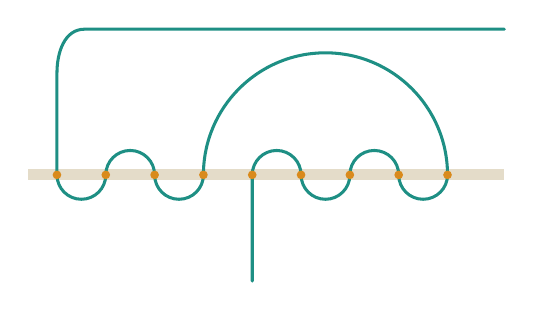
\begin{tikzpicture}[baseline=0pt]
\fill[road] (-0.372,-0.07) rectangle (5.682,0.07);
\draw[river] (2.480,-1.35) -- (2.480,0) arc (180:0:0.310) arc (180:360:0.310) arc (180:0:0.310) arc (180:360:0.310) arc (0:180:1.550) arc (360:180:0.310) arc (0:180:0.310) arc (360:180:0.310) -- (0.000,1.295) to[out=90,in=180] (0.350,1.850) -- (5.682,1.850);
\fill[bridge] (0.000,0) circle (0.055);
\fill[bridge] (0.620,0) circle (0.055);
\fill[bridge] (1.240,0) circle (0.055);
\fill[bridge] (1.860,0) circle (0.055);
\fill[bridge] (2.480,0) circle (0.055);
\fill[bridge] (3.100,0) circle (0.055);
\fill[bridge] (3.720,0) circle (0.055);
\fill[bridge] (4.340,0) circle (0.055);
\fill[bridge] (4.960,0) circle (0.055);
\end{tikzpicture}

\caption{One of the $262$ open meanders with $n=9$ crossings; its crossing order is $456783210$.}\label{fig:n9}
\end{figure}

\subsection{All implementations}\label{sec:implementations}
The repository contains the algorithms in five languages. Only the Lean programs are verified;
the others run the same machine and are checked against the certified values and the OEIS.

\begin{itemize}
  \item \emph{Lean.} The specification (evaluable by brute force for $n \le 6$), the search
    \code{meanderCount} with its array implementation substituted by \code{csimp}, and the
    transfer matrix in two variants: \code{tmCount}, compiled into the executable
    \code{meanders}, and \code{tmCountK}, evaluated by the kernel.
  \item \emph{Rust} (\code{rust/}). The transfer matrix with a packed state. Read along the cut
    from top to bottom, the open arcs pair up like brackets, because the pieces of river west of
    the cut never cross. So a state is a bracket word with at most one marker for the arc that
    leads to the east end, plus the number of arcs above the road, and fits in 64 bits for
    $n \le 52$. Each layer is split into 4096 hash shards, each an open-addressing table behind
    its own lock; worker threads claim source shards, batch successors per target shard, and
    free each source shard once read, so memory holds about one layer. Counts are kept modulo
    $2^{64}$ and, from $n = 44$, also modulo $2^{61}-1$, and recovered by the Chinese
    remainder theorem.
  \item \emph{OxCaml} (\code{oxcaml/}). The same algorithm in OxCaml, Jane Street's extension of
    OCaml. Workers run under OxCaml's \code{Parallel} scheduler, shards are capsules guarded by
    mutexes, and the compiler's mode system rules out data races. The state is an immediate
    63-bit integer, the hot loop allocates nothing on the heap, and tables are flat arrays of
    unboxed values that the garbage collector never scans.
  \item \emph{Python and OCaml.} Companion notebooks teach each language by building the
    specification, the parity search and the transfer matrix from scratch, with the state as
    a string or a list of constructors and layers in hash tables, run on all cores with process
    pools (Python) and domains (OCaml 5). A third notebook teaches Lean with the library's own
    declarations.
\end{itemize}

Table~\ref{tab:fast} times the parallel programs on a workstation with an 18-core Intel Xeon
W-2191B (36 threads) and 128~GB of memory, one value per run on all threads; on the same
machine the verified \code{meanders} computes all values up to $n=32$ in 160\,s. Every count
equals the OEIS term; in particular
\[
  \Open_{49} = 8{,}499{,}066{,}628{,}515{,}413{,}229{,}282, \qquad
  \Open_{50} = 22{,}206{,}891{,}674{,}746{,}169{,}557{,}410.
\]
Memory is the limit: the largest layer for $n = 50$ holds $2.25 \times 10^9$ states, and $n = 50$
is the largest value that fits in 128~GB, at about 35 bytes per state. Table~\ref{tab:scaling}
shows that both programs scale to the physical cores and no further, as expected for work
dominated by random memory access. On one thread the two are equally fast; OxCaml scales
better, probably because it pre-sizes each layer's tables so that a shard rarely grows while
its lock is held, at the cost of more memory. The teaching implementations are far slower:
interpreted Python computes all values up to $n = 30$ in about twelve seconds on the laptop, and the OCaml
notebook's transfer matrix, run as bytecode on ten domains, takes about half a second for
$n = 28$.

\begin{table}[t]
\centering
\begin{tabular}{rrrrr}
\toprule
$n$ & $\Open_n$ & largest layer & Rust & OxCaml \\
\midrule
40 & $1.66 \times 10^{17}$ & $2.2 \times 10^{7}$ & 3.3\,s & 2.3\,s \\
42 & $1.73 \times 10^{18}$ & $5.7 \times 10^{7}$ & 6.1\,s & 5.3\,s \\
44 & $1.83 \times 10^{19}$ & $1.4 \times 10^{8}$ & 30\,s & 25\,s \\
46 & $1.94 \times 10^{20}$ & $3.5 \times 10^{8}$ & 79\,s & 62\,s \\
49 & $8.50 \times 10^{21}$ & $1.4 \times 10^{9}$ & 516\,s & \\
50 & $2.22 \times 10^{22}$ & $2.3 \times 10^{9}$ & 1052\,s & \\
\bottomrule
\end{tabular}
\caption{The parallel programs on 36 threads of an 18-core Xeon with 128\,GB. From $n = 44$ a
value takes two sweeps. Peak memory at $n = 46$: 13.6\,GB (Rust), 22.9\,GB (OxCaml); at
$n = 50$: 79\,GB (Rust).}\label{tab:fast}
\end{table}

\begin{table}[t]
\centering
\begin{tabular}{lrrrrr}
\toprule
threads & 1 & 4 & 9 & 18 & 36 \\
\midrule
Rust   & 20.1\,s & 5.9\,s & 3.4\,s & 2.9\,s & 3.2\,s \\
OxCaml & 20.2\,s & 5.5\,s & 2.8\,s & 2.2\,s & 2.2\,s \\
\bottomrule
\end{tabular}
\caption{Scaling with threads for $n = 40$ on the same machine.}\label{tab:scaling}
\end{table}

\section{Discussion}

\subsection{What the proofs say about the algorithms}
The two pruning rules are the computational shadows of the Jordan curve theorem. Parity
(Lemma~\ref{lem:parity}) says that arcs pair up inside every region; viability says that a
point can close at most one arc per side. Neither rule needs any topology beyond the
interleaving of chords, which is why both proofs reduce to linear arithmetic.

The transfer-matrix proof is longer, mostly because the machine's state records connectivity
abstractly, by reference, while correctness needs to know what is connected to what. The
decorated machine bridges the gap: it carries explicit pieces of river, so the connectivity
argument becomes reasoning about lists. Making the abstract machine literally the decorated one
with decorations forgotten (\code{step\_abs}) means no separate refinement proof is needed.

\subsection{Meandric permutations and the conjectured scaling limit}\label{sec:permutons}
The specification is a statement about permutations, and the same permutations appear in recent
probability. Borga, Gwynne and Sun~\cite{bgs} attach to a closed meander its \emph{meandric
permutation}: number the crossings from west to east, and again in the order in which the
river meets them; the permutation relates the two orders. Up to inversion and the choice of
where and in which direction the river is started, this is the permutation $\sigma$ of
\code{IsClosedMeander}, and Rosenstiehl~\cite{rosenstiehl84} had studied the same objects as
planar permutations. The formalization therefore counts meandric permutations exactly, and
Theorem~\ref{thm:closed-open} is a bijection between meandric permutations of size $2n$ and
open meanders with $2n-1$ crossings.

Borga, Gwynne and Sun conjecture that a uniform random meander, viewed as a planar map with two
Hamiltonian paths (the road and the river), converges to a Liouville quantum gravity surface
with matter central charge $-4$, that is $\gamma = \sqrt{(17-\sqrt{145})/3} \approx 1.29$,
decorated by two independent space-filling SLE$_8$ curves, and that the plots of uniform
meandric permutations converge to the corresponding \emph{meandric permuton}. They prove, among
other things, that the longest increasing subsequence of permutations sampled from the
permuton is sublinear. The conjecture is the probabilistic counterpart of the asymptotic formula
of Di Francesco, Golinelli and Guitter~\cite{dgg00},
\[ \Closed_n \sim C\, A^n\, n^{-\alpha}, \qquad \alpha = \frac{29+\sqrt{145}}{12} \approx 3.4201, \]
for the number $\Closed_n$ of closed meanders of order $n$, with $A \approx 12.2629$ estimated by
Jensen and Guttmann~\cite{jensen00,jensen-guttmann}.

Exact counts test the exponent directly. With $A$ fixed at that estimate,
\[ \alpha_n = -\frac{\log\bigl(\Closed_{n+1}/(A \Closed_n)\bigr)}{\log(1 + 1/n)} \]
estimates $\alpha$, with an error of order $1/n$; extrapolating linearly in $1/n$ from $\alpha_{n-2}$ and $\alpha_n$ removes most
of it. Table~\ref{tab:exponent} uses $\Closed_n = \Open_{2n-1}$
(Theorem~\ref{thm:closed-open}) with open counts up to $49$ crossings, computed by the
parallel programs of Section~\ref{sec:implementations}. The
extrapolated values increase steadily towards $3.4201$. This is numerical evidence for the
conjectured exponent, not a proof, and it assumes the estimate of $A$.

\begin{table}[t]
\centering
\begin{tabular}{rrrr}
\toprule
$n$ & $\Closed_{n+1}/\Closed_n$ & $\alpha_n$ & extrapolated \\
\midrule
12 & 9.4415 & 3.2665 & 3.4053 \\
14 & 9.7747 & 3.2870 & 3.4100 \\
16 & 10.0377 & 3.3027 & 3.4129 \\
18 & 10.2506 & 3.3152 & 3.4149 \\
20 & 10.4263 & 3.3253 & 3.4163 \\
22 & 10.5739 & 3.3337 & 3.4172 \\
24 & 10.6996 & 3.3407 & 3.4180 \\
\midrule
\multicolumn{3}{r}{conjecture~\cite{dgg00}} & 3.4201 \\
\bottomrule
\end{tabular}
\caption{Estimates of the meander exponent $\alpha$ from exact counts of closed meanders, with
the growth constant fixed at $A = 12.2629$.}
\label{tab:exponent}
\end{table}

\subsection{Limitations and further work}
Our verified transfer matrix is far from the state of the art. Jensen's
algorithm~\cite{jensen00} encodes states more compactly and enumerates well beyond $n=32$. The
unverified Rust and OxCaml programs of Section~\ref{sec:implementations} pack each state into
one machine word and reach $n = 50$. Verifying such an encoding is a natural next step, and the generic counting theorem already accepts any merge procedure that preserves
weighted sums. A second direction is to formalize the rigorous growth-rate bounds of
Albert and Paterson~\cite{albert-paterson}, which would make our Catalan bound one instance of
a more general framework. Finally, the question that motivated the work, a closed formula for
the meander numbers, remains open; the conjectured critical exponent
$\alpha = (29+\sqrt{145})/12$ suggests that if a formula exists it is not of an elementary kind.

\subsection*{Acknowledgements}
The formalization and this paper were developed with the assistance of Claude Code (Anthropic).

\begin{thebibliography}{99}

\bibitem{albert-paterson}
M.~H.~Albert and M.~S.~Paterson, \emph{Bounds for the growth rate of meander numbers},
J.~Combin.\ Theory Ser.~A \textbf{112} (2005), 250--262.

\bibitem{arnold88}
V.~I.~Arnold, \emph{The branched covering $\mathbb{CP}^2 \to S^4$, hyperbolicity and
projective topology}, Siberian Math.~J.\ \textbf{29} (1988), 717--726.

\bibitem{bgs}
J.~Borga, E.~Gwynne and X.~Sun, \emph{Permutons, meanders, and SLE-decorated Liouville quantum
gravity}, J.~Eur.\ Math.\ Soc.\ \textbf{28} (2026), 4893--4949; arXiv:2207.02319.

\bibitem{dgg97}
P.~Di~Francesco, O.~Golinelli and E.~Guitter, \emph{Meander, folding, and arch statistics},
Math.\ Comput.\ Modelling \textbf{26} (1997), 97--147.

\bibitem{dgg00}
P.~Di~Francesco, O.~Golinelli and E.~Guitter, \emph{Meanders: exact asymptotics}, Nuclear
Phys.~B \textbf{570} (2000), 699--712.

\bibitem{jensen00}
I.~Jensen, \emph{A transfer matrix approach to the enumeration of plane meanders}, J.~Phys.~A
\textbf{33} (2000), 5953--5963.

\bibitem{jensen-guttmann}
I.~Jensen and A.~J.~Guttmann, \emph{Critical exponents of plane meanders}, J.~Phys.~A
\textbf{33} (2000), L187--L192.

\bibitem{lando-zvonkin}
S.~K.~Lando and A.~K.~Zvonkin, \emph{Plane and projective meanders}, Theoret.\ Comput.\ Sci.\
\textbf{117} (1993), 227--241.

\bibitem{lean4}
L.~de~Moura and S.~Ullrich, \emph{The Lean~4 theorem prover and programming language}, in
Automated Deduction -- CADE~28, Lecture Notes in Comput.\ Sci.\ \textbf{12699}, Springer, 2021,
625--635.

\bibitem{mathlib}
The mathlib Community, \emph{The Lean mathematical library}, in Proceedings of the 9th ACM
SIGPLAN International Conference on Certified Programs and Proofs (CPP 2020), 367--381.

\bibitem{oeis-a005316}
OEIS Foundation, \emph{Sequence A005316: Meandric numbers}, The On-Line Encyclopedia of
Integer Sequences, \url{https://oeis.org/A005316}.

\bibitem{oeis-a005315}
OEIS Foundation, \emph{Sequence A005315: Closed meandric numbers}, The On-Line Encyclopedia of
Integer Sequences, \url{https://oeis.org/A005315}.

\bibitem{rosenstiehl84}
P.~Rosenstiehl, \emph{Planar permutations defined by two intersecting Jordan curves}, in Graph
Theory and Combinatorics (Cambridge, 1983), Academic Press, London, 1984, 259--271.

\bibitem{touchard50}
J.~Touchard, \emph{Contributions \`a l'\'etude du probl\`eme des timbres-poste}, Canad.\
J.~Math.\ \textbf{2} (1950), 385--398.

\end{thebibliography}

\end{document}
